\documentclass[tikz,border=8pt]{standalone}
% Shared look for every TikZ diagram. Load with \input{../../tools/tikz-style.tex}
\usepackage[T1]{fontenc}
\usepackage{lmodern}
\renewcommand{\sfdefault}{lmr}  % diagrams use the same serif as the text
\usetikzlibrary{arrows.meta, positioning, shapes.geometric, calc, fit, backgrounds}
\definecolor{cblue}{HTML}{4C78A8}
\definecolor{corange}{HTML}{F58518}
\definecolor{cgreen}{HTML}{54A24B}
\definecolor{cred}{HTML}{E45756}
\definecolor{cpurple}{HTML}{B279A2}
\definecolor{cgrey}{HTML}{6B6B6B}
\tikzset{
  every picture/.style={font=\sffamily, line width=1.2pt},
  box/.style={draw=#1, fill=#1!12, rounded corners=4pt, align=center, inner sep=7pt, minimum height=1.1cm},
  box/.default=cgrey,
  arrow/.style={-{Stealth[length=3mm]}, draw=cgrey, line width=1.4pt},
  title/.style={font=\sffamily\bfseries\Large},
  note/.style={font=\sffamily\small, text=cgrey, align=center},
}
\AtBeginDocument{\hyphenpenalty=10000 \exhyphenpenalty=10000}

\begin{document}
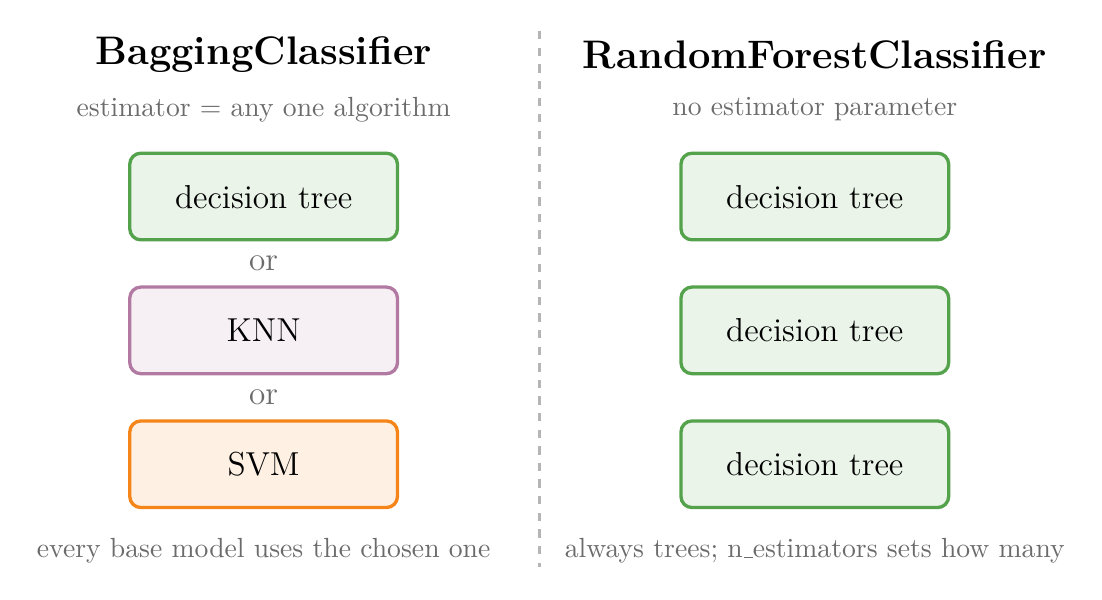
\begin{tikzpicture}[m/.style={box=#1, minimum width=3.4cm, font=\sffamily\large}]
  \node[title] at (0,2.4) {BaggingClassifier};
  \node[note, font=\sffamily\normalsize] at (0,1.7) {estimator = any one algorithm};
  \node[m=cgreen] at (0,0.6) {decision tree};
  \node[font=\sffamily\large, text=cgrey] at (0,-0.25) {or};
  \node[m=cpurple] at (0,-1.1) {KNN};
  \node[font=\sffamily\large, text=cgrey] at (0,-1.95) {or};
  \node[m=corange] at (0,-2.8) {SVM};
  \node[title] at (7,2.4) {RandomForestClassifier};
  \node[note, font=\sffamily\normalsize] at (7,1.7) {no estimator parameter};
  \node[m=cgreen] at (7,0.6) {decision tree};
  \node[m=cgreen] at (7,-1.1) {decision tree};
  \node[m=cgreen] at (7,-2.8) {decision tree};
  \node[note, font=\sffamily\normalsize] at (7,-3.9) {always trees; n\_estimators sets how many};
  \node[note, font=\sffamily\normalsize] at (0,-3.9) {every base model uses the chosen one};
  \draw[cgrey!50, dashed] (3.5,2.7) -- (3.5,-4.1);
\end{tikzpicture}
\end{document}
